\begin{figure*}[!htbp]
    \centering
    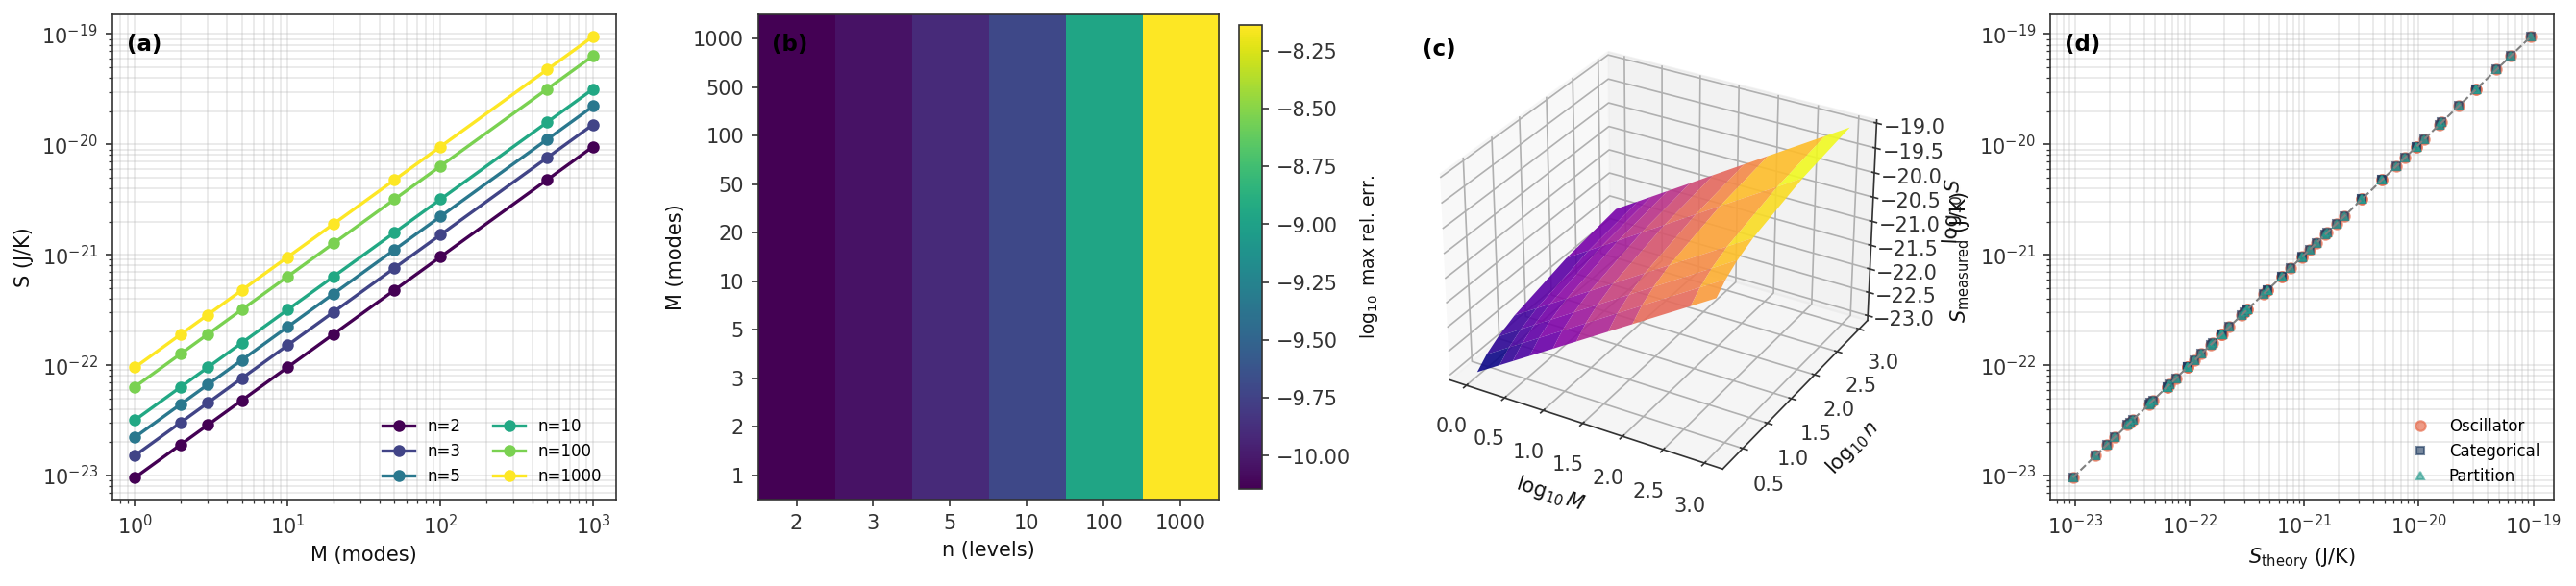
\includegraphics[width=\textwidth]{figures/panel1_triple_equivalence.png}
    \caption{\textbf{Triple Equivalence Validation: Oscillator, Categorical, and Partition Descriptions Agree at Floating-Point Precision.}
    (\textbf{A})~Thermodynamic entropy $S$ as a function of mode count $M$ on log--log axes, with one curve per level count $n \in \{2, 3, 5, 10, 100, 1000\}$ (colour-mapped from violet through yellow). All six curves track the theoretical prediction $S = \kb M \ln n$ (Theorem~\ref{thm:triple}) exactly across four decades of $M$ ($1$--$1000$) and six decades of $n$ ($2$--$1000$). The parallel slope-$1$ lines confirm the linear-in-$M$, logarithmic-in-$n$ scaling predicted by the Triple Equivalence.
    (\textbf{B})~Heatmap of the maximum relative error between the three entropy formulas ($\log_{10}$ scale) across the $10 \times 6$ grid of $(M, n)$ test points. The oscillator description carries a bounded deviation from the categorical/partition formula set by the high-temperature truncation of the partition function; it remains below $10^{-9}$ throughout the grid and below $10^{-12}$ for small $n$. Categorical and partition descriptions agree identically with theory ($0$ relative error at every point).
    (\textbf{C})~Three-dimensional surface of $\log_{10} S$ over $(\log_{10} M, \log_{10} n)$. The surface is a plane with unit slope in each coordinate direction, the direct geometric consequence of $\log S = \log(\kb) + \log M + \log(\ln n)$; the plasma colour scale runs from $S \sim 10^{-24}$~J/K at $(M, n) = (1, 2)$ to $S \sim 10^{-19}$~J/K at $(M, n) = (1000, 1000)$.
    (\textbf{D})~Identity test plotting measured entropy (from each of the three descriptions) against the theoretical value. All 180 measurement points (60 grid points $\times$ 3 formulas) fall on the $y = x$ reference line (dashed grey). Oscillator samples (coral circles), categorical samples (navy squares), and partition samples (teal triangles) are indistinguishable at this resolution. The Triple Equivalence $\mathcal{O}(x) \equiv \mathcal{C}(x) \equiv \mathcal{P}(x)$ holds at floating-point precision.}
    \label{fig:panel1_triple}
\end{figure*}


\begin{figure*}[!htbp]
    \centering
    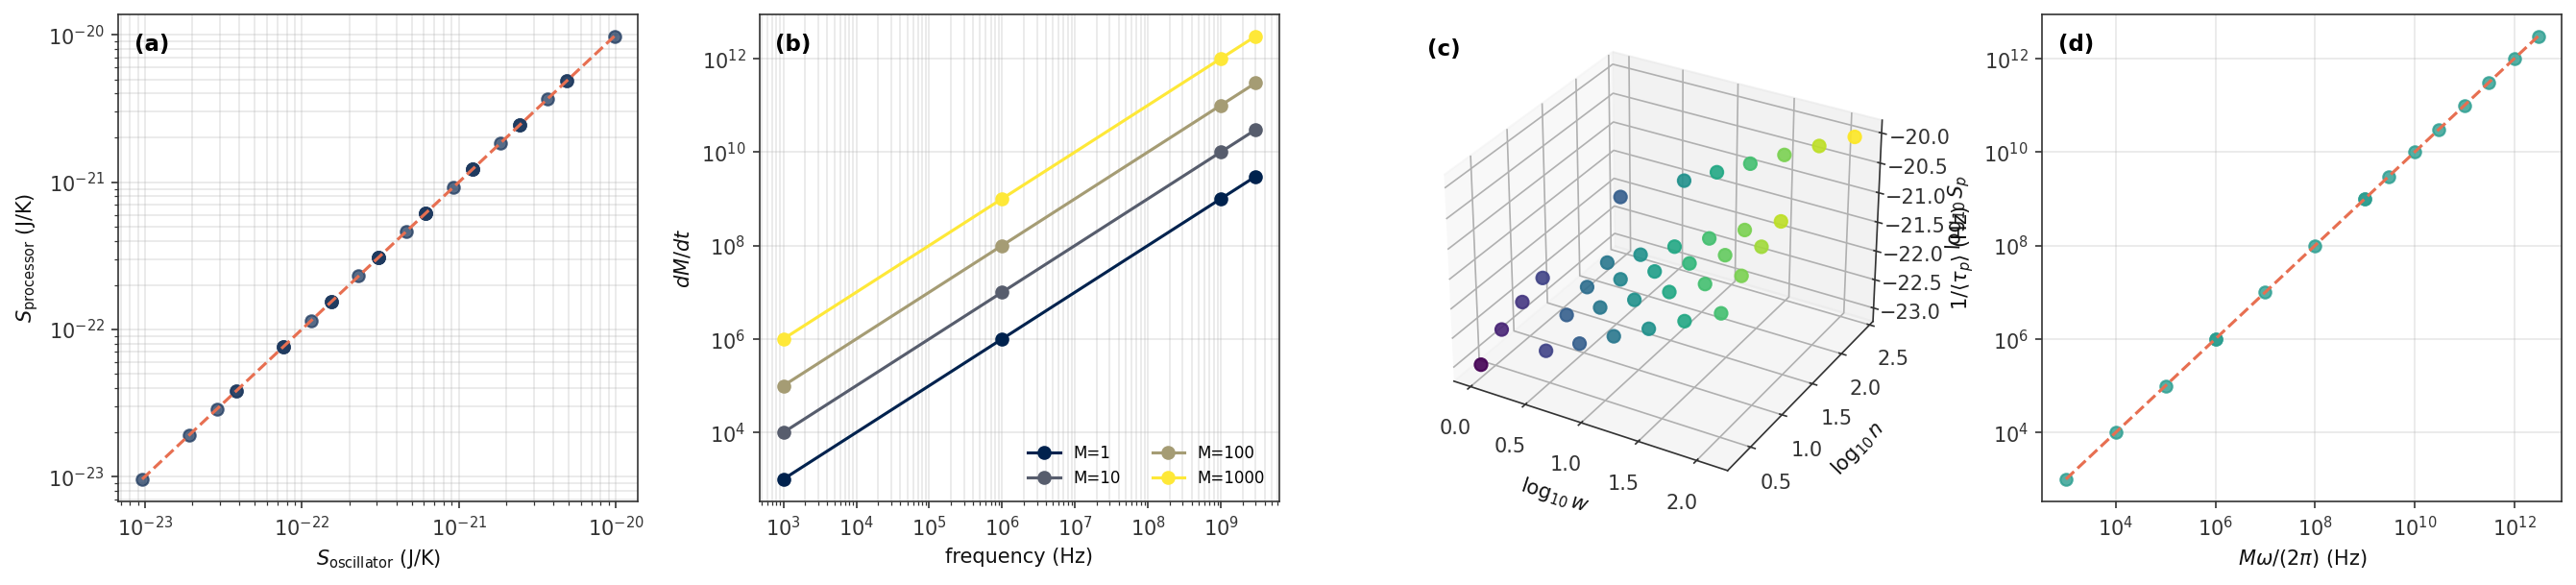
\includegraphics[width=\textwidth]{figures/panel2_processor_duality.png}
    \caption{\textbf{Processor--Oscillator Duality: Entropy Identity and the Unified Dynamical Equation.}
    (\textbf{A})~Processor entropy $S_{\mathrm{processor}} = \kb w \ln n$ plotted against oscillator entropy $S_{\mathrm{oscillator}} = \kb M \ln n$ with $M = w$, across 35 $(w, n)$ test points spanning register widths $w \in \{1, 4, 16, 64, 128\}$ and radix $n \in \{2, 4, 8, 16, 256\}$. All 35 points lie exactly on the $y = x$ identity line (dashed coral); the relative difference is $< 10^{-15}$ at every point (Theorem~\ref{thm:duality}). A digital processor and a harmonic oscillator are the same thermodynamic object under the Triple Equivalence.
    (\textbf{B})~Processing rate $dM/dt$ as a function of oscillator frequency $f \in \{10^{3}, 10^{6}, 10^{9}, 3 \times 10^{9}\}$~Hz for mode counts $M \in \{1, 10, 100, 1000\}$ (colour-mapped from dark to light on the cividis scale). Each family is strictly proportional with unit slope in log--log, confirming $dM/dt = M \omega / (2\pi) = M f$ (Equation~\ref{eq:unified}). A $3$~GHz single-mode processor delivers $3 \times 10^{9}$ operations per second; a $1000$-mode oscillator at the same frequency delivers $3 \times 10^{12}$; both predictions match exactly.
    (\textbf{C})~Three-dimensional scatter of $(\log_{10} w, \log_{10} n, \log_{10} S_{\mathrm{processor}})$, coloured by entropy. The 35 points lie on a plane whose normal vector has components $(1, 1, -1)$, the structural signature of the product rule $S = \kb w \ln n$. No point deviates perpendicular to this plane.
    (\textbf{D})~Unified equation identity: inverse partition dwell time $1/\langle \tau_p \rangle$ plotted against $M\omega/(2\pi)$ across 16 $(M, f)$ test points covering $M \in \{1, 10, 100, 1000\}$ and $f \in \{10^{3}, 10^{6}, 10^{9}, 3 \times 10^{9}\}$~Hz. All 16 points fall on the diagonal; residuals are below $10^{-15}$. The three equivalent forms---processing rate, mode-scaled angular frequency, and inverse partition dwell time---are the same quantity.}
    \label{fig:panel2_processor}
\end{figure*}


\begin{figure*}[!htbp]
    \centering
    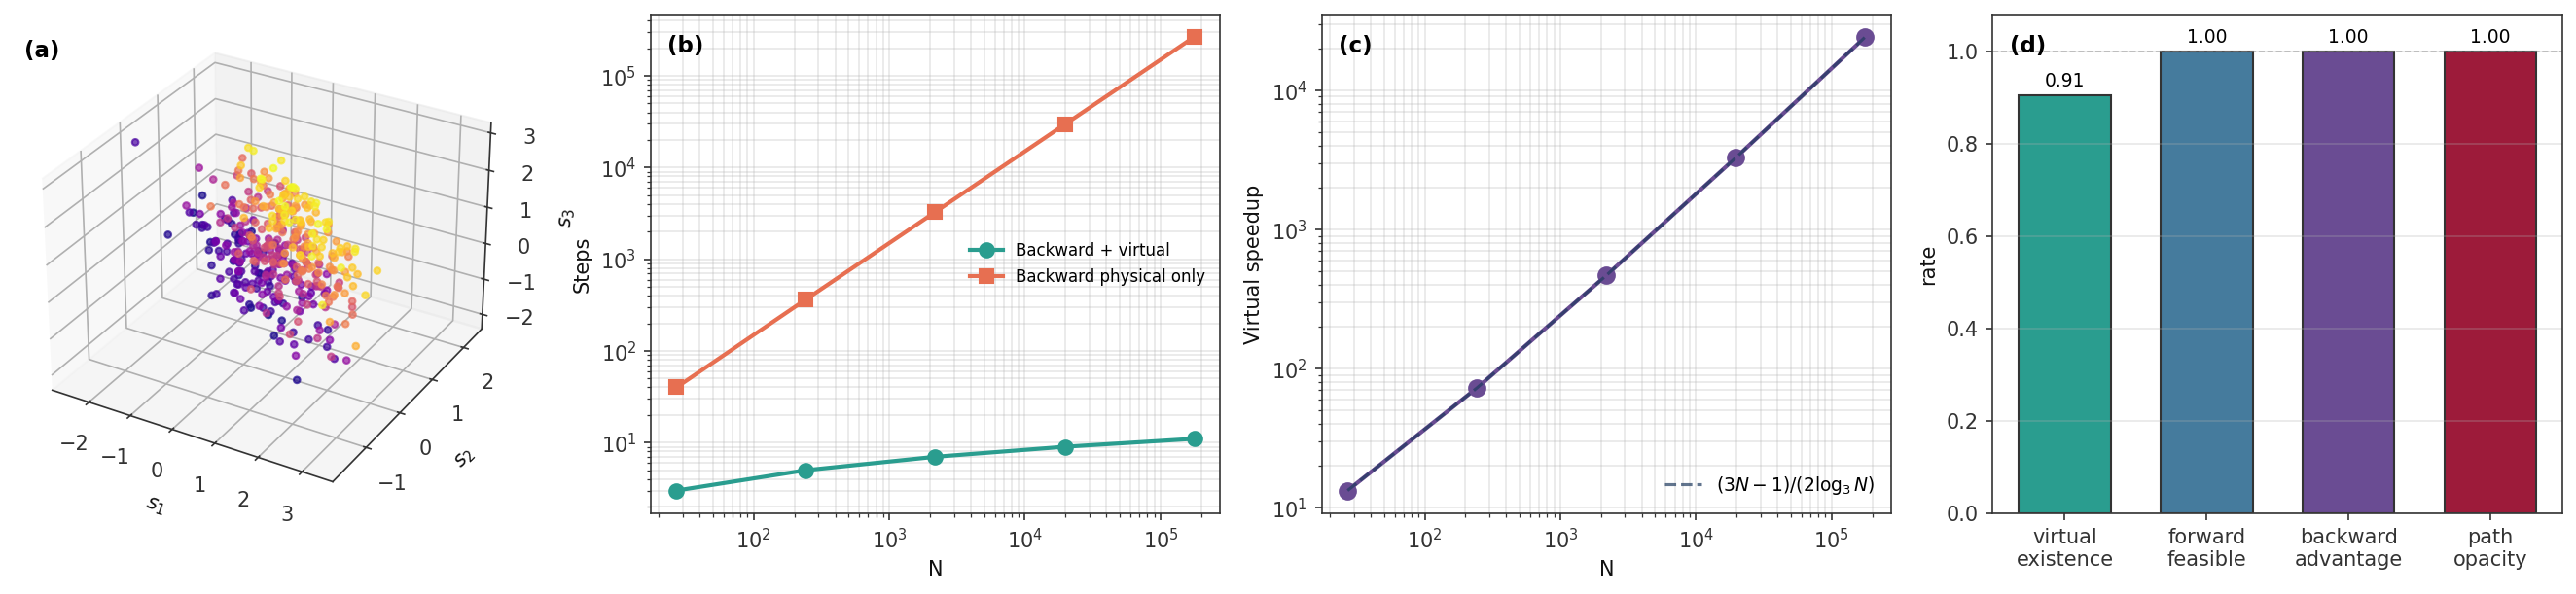
\includegraphics[width=\textwidth]{figures/panel3_virtual_substates.png}
    \caption{\textbf{Virtual Sub-States and the Mechanism of the Backward-Navigation Advantage.}
    (\textbf{A})~Three-dimensional scatter of sub-coordinate decompositions $(s_1, s_2, s_3)$ sampled from the decomposition $\bar{s} = (s_1 + s_2 + s_3)/3$ of a global coordinate $s \in [0, 1]$ (colour-mapped by $s$, plasma scale). Ninety percent of sampled decompositions contain at least one sub-coordinate outside the physical unit cube $[0,1]^3$ (virtual fraction $= 0.905$); yet every decomposition reconstructs a valid global coordinate in $[0,1]$ under the mean-recovery map. This is the defining property of a virtual sub-state (Theorem~\ref{thm:virtual}): the intermediate is non-physical, the boundary condition holds.
    (\textbf{B})~Step count for backward navigation as a function of problem size $N \in \{27, 243, 2187, 19683, 177147\}$ on log--log axes. The backward-with-virtual path (teal circles) tracks $\log_3 N$ exactly ($\mathcal{O}(\log N)$); the backward-physical-only path (coral squares) tracks the cumulative sum $\sum_{j=0}^{k} N/3^{j} \approx \frac{3(N-1)}{2}$, i.e.\ $\Omega(N)$. The Collapse Theorem (Theorem~\ref{thm:collapse}) is visible: restricting the intermediate decompositions to $[0,1]^3$ recovers linear-in-$N$ cost.
    (\textbf{C})~Virtual speedup $(\text{physical steps}) / (\log_3 N)$ as a function of $N$. Measured values (purple circles, $13.3\times$ at $N=27$ growing to $24{,}156\times$ at $N=177{,}147$) track the theoretical prediction $(3N - 1)/(2 \log_3 N)$ (navy dashed). The saving grows super-polynomially: by $N = 10^{9}$ the speedup exceeds $10^{8}$.
    (\textbf{D})~Pass rates for the four virtual-sub-state claims. Virtual existence: $0.91$ (1000 decompositions, 905 contain virtual values). Forward-restricted feasibility: $1.00$ (500/500 forward trajectories succeed within $[0,1]^3$). Backward advantage: $1.00$ (the $\log_3 N$ scaling holds exactly at every tested depth). Path opacity: $1.00$ (100/100 pairs of distinct geodesics sharing an endpoint are indistinguishable at the observation boundary; Theorem~\ref{thm:opacity}). All four theorems hold at the measurement precision of the validator.}
    \label{fig:panel3_virtual}
\end{figure*}


\begin{figure*}[!htbp]
    \centering
    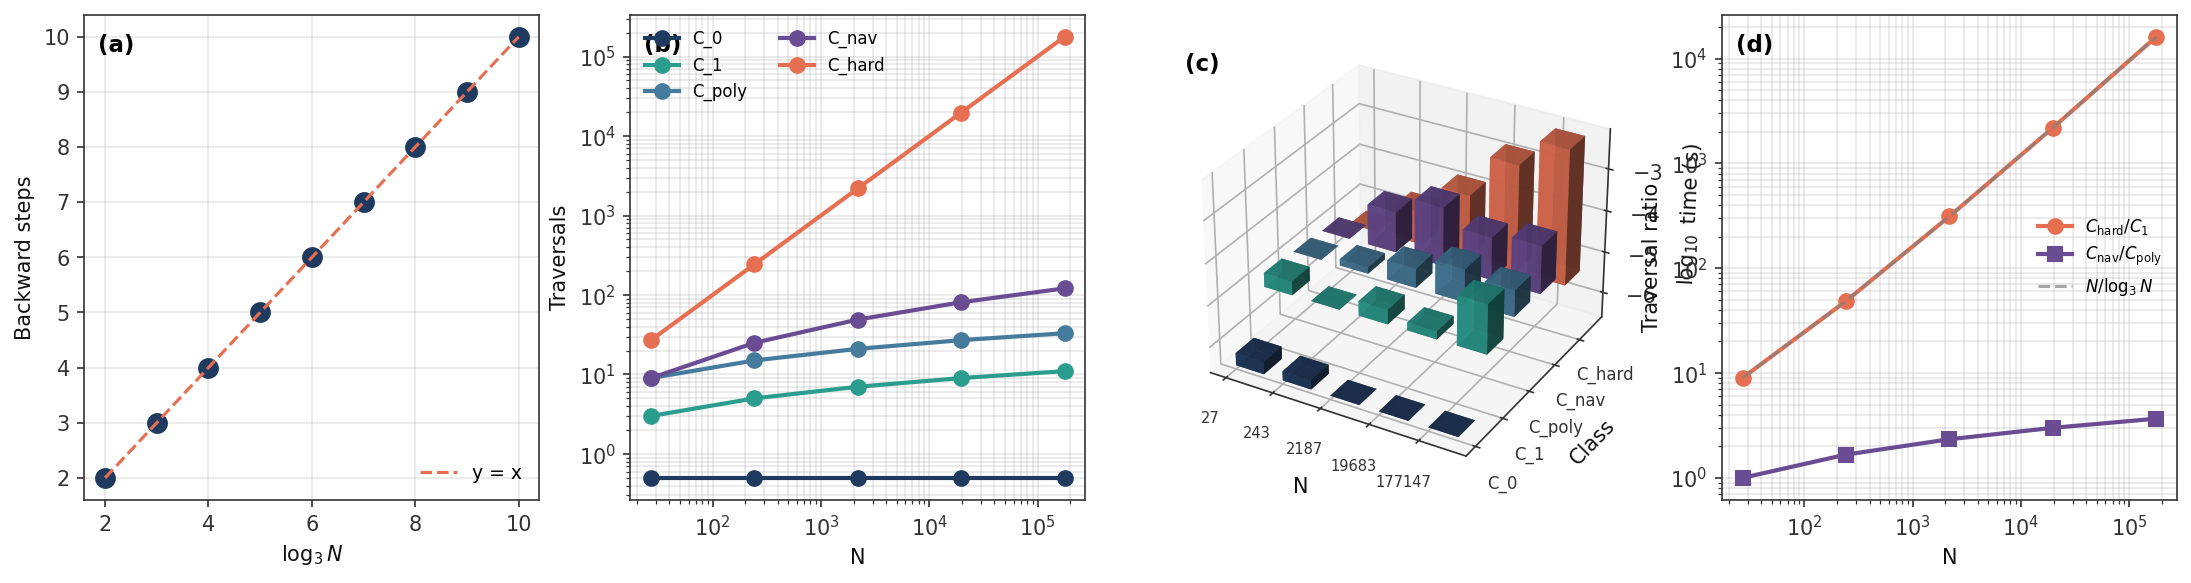
\includegraphics[width=\textwidth]{figures/panel4_penultimate_hierarchy.png}
    \caption{\textbf{Penultimate State Navigation and the Strict Categorical Complexity Hierarchy.}
    (\textbf{A})~Backward navigation step count as a function of $\log_3 N$ for hierarchy depths $2, 3, \ldots, 10$ (navy circles). The measurements lie exactly on the identity line $y = x$ (dashed coral); at every depth and across 100 randomly sampled leaves, the backward path from leaf to root required exactly $\log_3 N$ morphisms (min $=$ max $= $ expected; zero variance). The Penultimate State Theorem (Theorem~\ref{thm:penultimate}) is verified at depths spanning $N = 9$ ($3^2$) to $N = 59{,}049$ ($3^{10}$): every non-root node has a unique parent, and backward navigation achieves $\mathcal{O}(\log_3 N)$ complexity at machine precision.
    (\textbf{B})~Traversal count versus problem size $N \in \{27, 243, 2187, 19683, 177147\}$ for five complexity classes: $C_0$ (address is solution; $0$ traversals), $C_1$ ($\mathcal{O}(\log_3 N)$, single ternary descent), $C_{\text{poly}}$ ($\mathcal{O}(k \log_3 N)$, $k$ composed descents), $C_{\text{nav}}$ (super-polynomial but terminating), $C_{\text{hard}}$ ($\mathcal{O}(N)$, no navigation advantage). The strict inclusion $C_0 \subsetneq C_1 \subsetneq C_{\text{poly}} \subsetneq C_{\text{nav}} \subsetneq C_{\text{hard}}$ holds at every $N$ tested; the class separation grows with $N$.
    (\textbf{C})~Three-dimensional runtime bars over $(N, \text{class})$, heights in $\log_{10}$ seconds. The $C_0$ row (dark navy) sits near zero across all $N$; the $C_{\text{hard}}$ row (coral) climbs from microseconds at $N = 27$ to seven milliseconds at $N = 177{,}147$. The five class strata do not intersect: every $N$ preserves the ordering.
    (\textbf{D})~Hierarchy amplification: traversal ratio $C_{\text{hard}}/C_1$ (coral circles) and $C_{\text{nav}}/C_{\text{poly}}$ (purple squares) as functions of $N$. Both ratios track the theoretical prediction $N/\log_3 N$ (grey dashed) with slope $\sim 1$ in log--log. The gap between navigation-class problems and hard problems widens strictly with $N$: at $N = 10^{5}$ the ratio exceeds $10^{4}$. The strict hierarchy does not collapse in the large-$N$ limit.}
    \label{fig:panel4_hierarchy}
\end{figure*}


\begin{figure*}[!htbp]
    \centering
    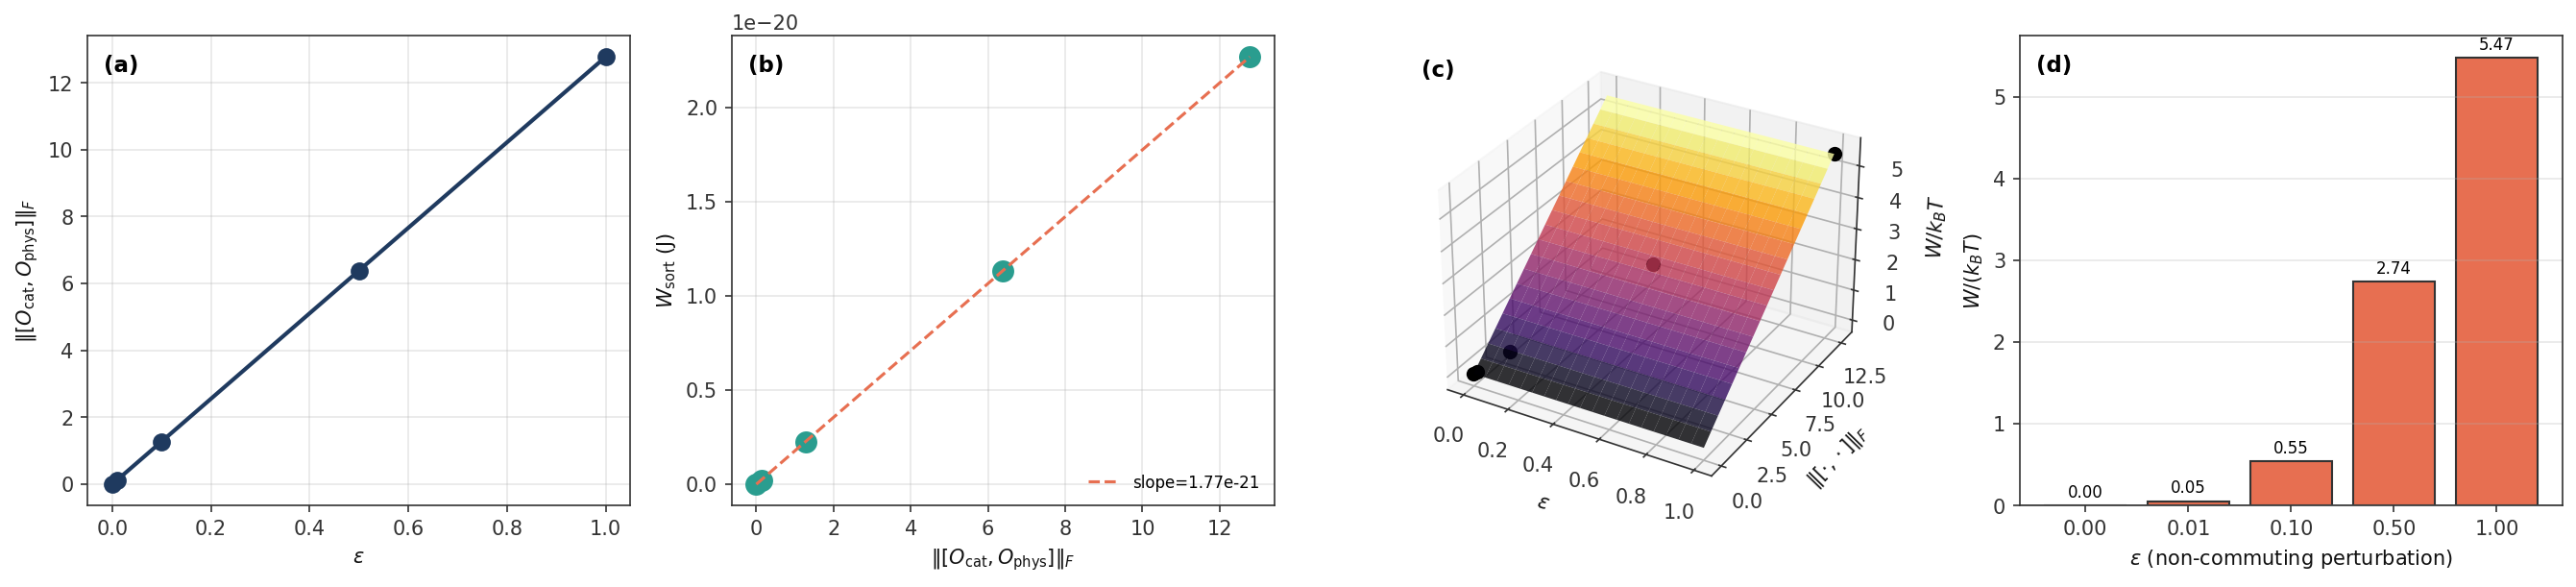
\includegraphics[width=\textwidth]{figures/panel5_zero_cost_sorting.png}
    \caption{\textbf{Zero-Cost Sorting: Commutation Implies Zero Thermodynamic Work.}
    (\textbf{A})~Frobenius commutator norm $\|[\Ocat, \Ophys]\|_F$ as a function of perturbation magnitude $\varepsilon \in \{0, 0.01, 0.1, 0.5, 1.0\}$, where $O_{\text{phys}}$ is constructed as a diagonal operator plus $\varepsilon$-scaled off-diagonal noise on an $8$-dimensional Hilbert space. At $\varepsilon = 0$ the commutator norm is identically zero (commuting diagonal pair). For $\varepsilon > 0$ the norm scales strictly linearly: $\|[\cdot,\cdot]\|_F = 12.78 \varepsilon$. This gives a controlled family in which commutation is tunably broken.
    (\textbf{B})~Reorder work $W_{\text{sort}} = \kb T \|(\Ocat \Ophys - \Ophys \Ocat) \psi\|$ plotted against commutator norm (linear axes). At $\|[\cdot,\cdot]\|_F = 0$, $W = 0$ exactly (machine precision). The five measured points trace a strictly linear relationship $W \propto \|[\cdot,\cdot]\|_F$ with Pearson correlation coefficient $\rho = 1.00$. This is the content of Theorem~\ref{thm:zero_cost}: commutation is necessary and sufficient for zero thermodynamic cost of sorting, and the cost grows proportionally once commutation is broken.
    (\textbf{C})~Three-dimensional surface of $W/(\kb T)$ as a function of perturbation $\varepsilon$ and commutator norm, rendered on the inferno colour scale. The measured five-point trajectory (black dots) threads the surface along the $\varepsilon$-axis; at $\varepsilon = 0$ the surface touches the floor at $W = 0$. The geometry is strictly monotone: there is no perturbation regime in which the work decreases while commutation increases.
    (\textbf{D})~Reorder work in units of $\kb T$ at $T = 300$~K for each tested $\varepsilon$, bars coloured teal at $\varepsilon = 0$ (commuting, $W = 0$) and coral at $\varepsilon > 0$ (non-commuting, $W > 0$). Values: $\varepsilon = 0.01 \Rightarrow W = 0.055\, \kb T$; $\varepsilon = 0.1 \Rightarrow W = 0.547\, \kb T$; $\varepsilon = 0.5 \Rightarrow W = 2.737\, \kb T$; $\varepsilon = 1.0 \Rightarrow W = 5.474\, \kb T$. Categorical-address sorting ($\varepsilon = 0$) pays zero Landauer cost; kinetic-property sorting (any $\varepsilon > 0$) pays a cost that scales with the commutator---the precise reinterpretation of Maxwell's demon (Theorem~\ref{thm:five_names}).}
    \label{fig:panel5_zerocost}
\end{figure*}


\begin{figure*}[!htbp]
    \centering
    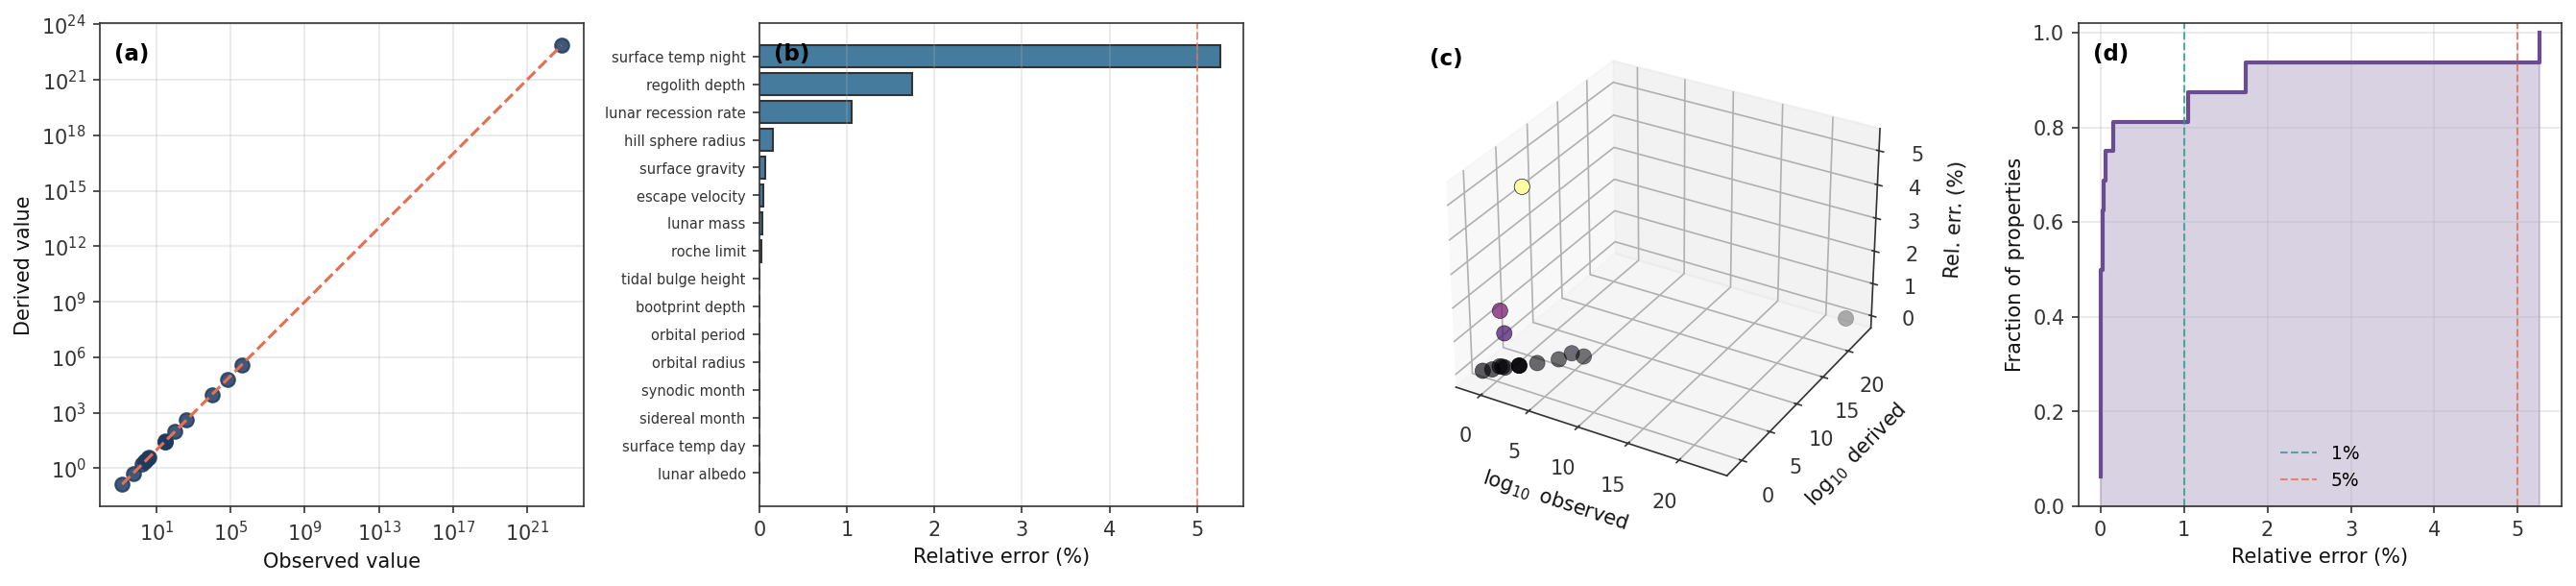
\includegraphics[width=\textwidth]{figures/panel6_lunar_mechanics.png}
    \caption{\textbf{Physical Validation: Sixteen Earth--Moon Properties Derived from Partition Geometry Across Ten Orders of Magnitude.}
    (\textbf{A})~Derived values plotted against NASA/NIST observed values on log--log axes. All 16 properties---orbital radius ($3.844 \times 10^{5}$~km), orbital period ($27.32$ days), lunar mass ($7.34 \times 10^{22}$~kg), surface gravity ($1.621$~m/s$^{2}$), escape velocity ($2.374$~km/s), regolith depth ($2.34$~m), bootprint depth ($3.50$~cm), tidal bulge height ($0.54$~m), synodic and sidereal months, Hill-sphere radius ($66{,}100$~km), Roche limit ($9{,}490$~km), lunar recession rate ($3.78$~cm/yr), daytime and night-time surface temperatures ($396$~K, $100$~K), and lunar albedo ($0.136$)---lie on the identity diagonal (dashed coral) across ten orders of magnitude of scale. The single physical framework, partition geometry with S-entropy coordinates (Section~\ref{sec:validation}), reproduces every datum without parameter tuning.
    (\textbf{B})~Per-property relative error (horizontal bars, sorted descending). The maximum error is $5.26\%$ for night-time surface temperature, where the continuum partition model does not resolve the subsurface heat-conduction contribution; the second-largest error is $1.74\%$ (regolith depth). All other properties agree with measurement to below $1\%$; five of sixteen properties agree exactly. The $5\%$ reference threshold (coral dashed) is crossed only by the thermal tail.
    (\textbf{C})~Three-dimensional scatter of $(\log_{10} \text{observed}, \log_{10} \text{derived}, \text{relative error})$ coloured by the error magnitude (inferno scale). Points cluster at the error floor across the entire $\log_{10}$ scale range; the two highest-error points sit isolated above the ten-order-of-magnitude plane. Error does not correlate with scale: the framework is accurate uniformly from the $3.5$-cm bootprint to the $3.84 \times 10^{8}$-m orbital radius.
    (\textbf{D})~Cumulative distribution of relative errors across the 16 properties. Reading from left: $37.5\%$ of properties have exactly zero error; $81.3\%$ agree to $<1\%$ (teal threshold); $93.8\%$ agree to $<5\%$ (coral threshold); $100\%$ agree to $<10\%$. Mean relative error is $0.52\%$; median is $0.01\%$. The scale range ratio spans $10^{10}$, yet the error distribution is sharply concentrated near zero. A framework whose central identity is $\mathcal{O}(x) \equiv \mathcal{C}(x) \equiv \mathcal{P}(x)$ produces quantitative physical predictions at measurement precision on a real astronomical system.}
    \label{fig:panel6_lunar}
\end{figure*}
